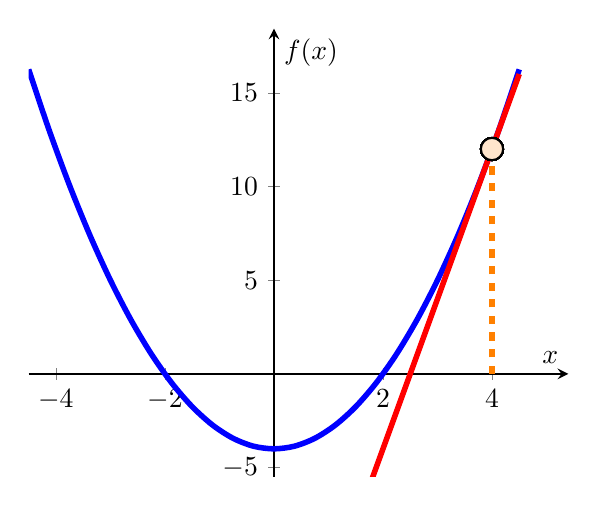
\begin{tikzpicture}
\begin{axis}[axis lines=middle, line width=0.7, enlargelimits=upper, domain=-4.5:4.5, ymin=-5.5, xlabel=$x$, ylabel=$f(x)$]
\addplot [smooth, color=blue, line width = 2] {x^2-4};
\addplot[smooth, color=orange, dashed, line width = 2] coordinates {(4,0) (4,12)};
\addplot[only marks, mark size=4, color=orange!20, draw=black] (4,12);
\addplot [smooth, color=red, line width = 2] {8*x-20};
\end{axis}
\end{tikzpicture}